
\begin{flushleft}

\chapter{Establishing Unicast connection between 2 XBee modules}


\medskip
\section{\textbf{Installation of X-CTU (Windows)}}
\medskip
Hello world ! This is a quick installation tutorial for Digi's X-CTU software.
The X-CTU Software enables you to configure and test various kinds of communication modes between XBee modules.
\medskip
\subsection{\textbf{ System Requirements}}
\medskip
\begin{enumerate}
\item \textbf{Supported Operating Systems:} Windows 98, Windows ME, Windows 2K, Windows XP, Windows Vista, Windows 7, Windows 8, Windows 8.1

\item \textbf{Non-supported Operating Systems:} Windows 95, Windows NT, Linux

\item \textbf{Hardware Requirements:} 
\begin{enumerate}
\item 2 XBee modules
\item 1 XBee USB adapter 
\item Dedicated USB 2.0 bus
\item USB A-Type Male to USB B-Type Male Cable
\item Firebird V robot
\end{enumerate}
\end{enumerate}
\medskip

\subsection{\textbf{ Installation Procedure}}
\addcontentsline{lof}{figure}{\textbf{Installation Procedure of X-CTU}}
\textbf{Step 1 :}

\medskip

Launch Setup\_XCTU\_5260.exe to start installation of Digi's X-CTU software for configuration of XBee modules. Click "Next" to continue. Shown in figure \ref{zstep1}. 

\medskip

\textbf{Step 2 :}

\medskip

Read the license agreement and select the "I Agree" radio button if you wish to continue.Click "Next".
Shown in figure \ref{zstep2}.

\medskip

\textbf{Step 3 :}

\medskip


Select the installation folder you wish to install X-CTU to, and whether you wish to install for Everyone or just the current user.Click "Next".
Shown in figure \ref{zstep3}.

\medskip

\textbf{Step 4 :}

\medskip

Confirm the installation by clicking "Next".Shown in figure \ref{zstep4}.

\medskip

\textbf{Step 5 :}

\medskip

Wait till the installation is complete.
If you wish to check out Digi's website for firmware updates, click "Yes", else click "No". Shown in figure \ref{zstep5}.

\begin{figure}
\begin{center}
\includegraphics[scale=0.5]{zigbee_1}
\end{center}
\caption{Step 1 - Welcome to X-CTU Setup Wizard}
\label{zstep1}
\end{figure}
\medskip

\begin{figure}
\begin{center}
\includegraphics[scale=0.5]{zigbee_2}
\end{center}
\caption{Step 2 - License Agreement}
\label{zstep2}
\end{figure}
\medskip

\begin{figure}
\begin{center}
\includegraphics[scale=0.5]{zigbee_3}
\end{center}
\caption{Step 3 - Select Installation Folder}
\label{zstep3}
\end{figure}
\medskip

\newpage

\begin{figure}
\begin{center}
\includegraphics[scale=0.5]{zigbee_4}
\end{center}
\caption{Step 4 - Confirm Installation}
\label{zstep4}
\end{figure}
\medskip

\begin{figure}
\begin{center}
\includegraphics[scale=0.5]{zigbee_5}
\end{center}
\caption{Step 5 - Installing X-CTU}
\label{zstep5}
\end{figure}
\medskip


Congratulations! X-CTU was successfully installed if you followed the above steps correctly. Click "Close" to close the installation window.

\newpage

\subsection{\textbf{Configuring 2 XBee modules for unicast connection}}
\addcontentsline{lof}{figure}{\textbf{Configuring 2 XBee modules for unicast connection}}

Hello world ! This is a quick tutorial for configuration of 2 XBee modules for working in Unicast mode.

\medskip

\textbf{Step 1 :}

\medskip

Plug in an XBee module in the XBee USB adapter and connect it to a USB port of the PC. Launch X-CTU. Select the "USB Serial Port(COM3)" entry under the "Select Com Port" title. The COM port number varies according to hardware configuration. It might be different for you. Setup the COM port according to the settings shown in the figure. Shown in figures \ref{xstep1.1} and \ref{xstep1.2}.

\begin{figure}[h]
\begin{center}
\includegraphics[scale=0.5]{zigbee_8}
\end{center}
\caption{Step 1(a) - X-CTU User Interface}
\label{xstep1.1}
\end{figure}
\medskip

\begin{figure}[h]
\begin{center}
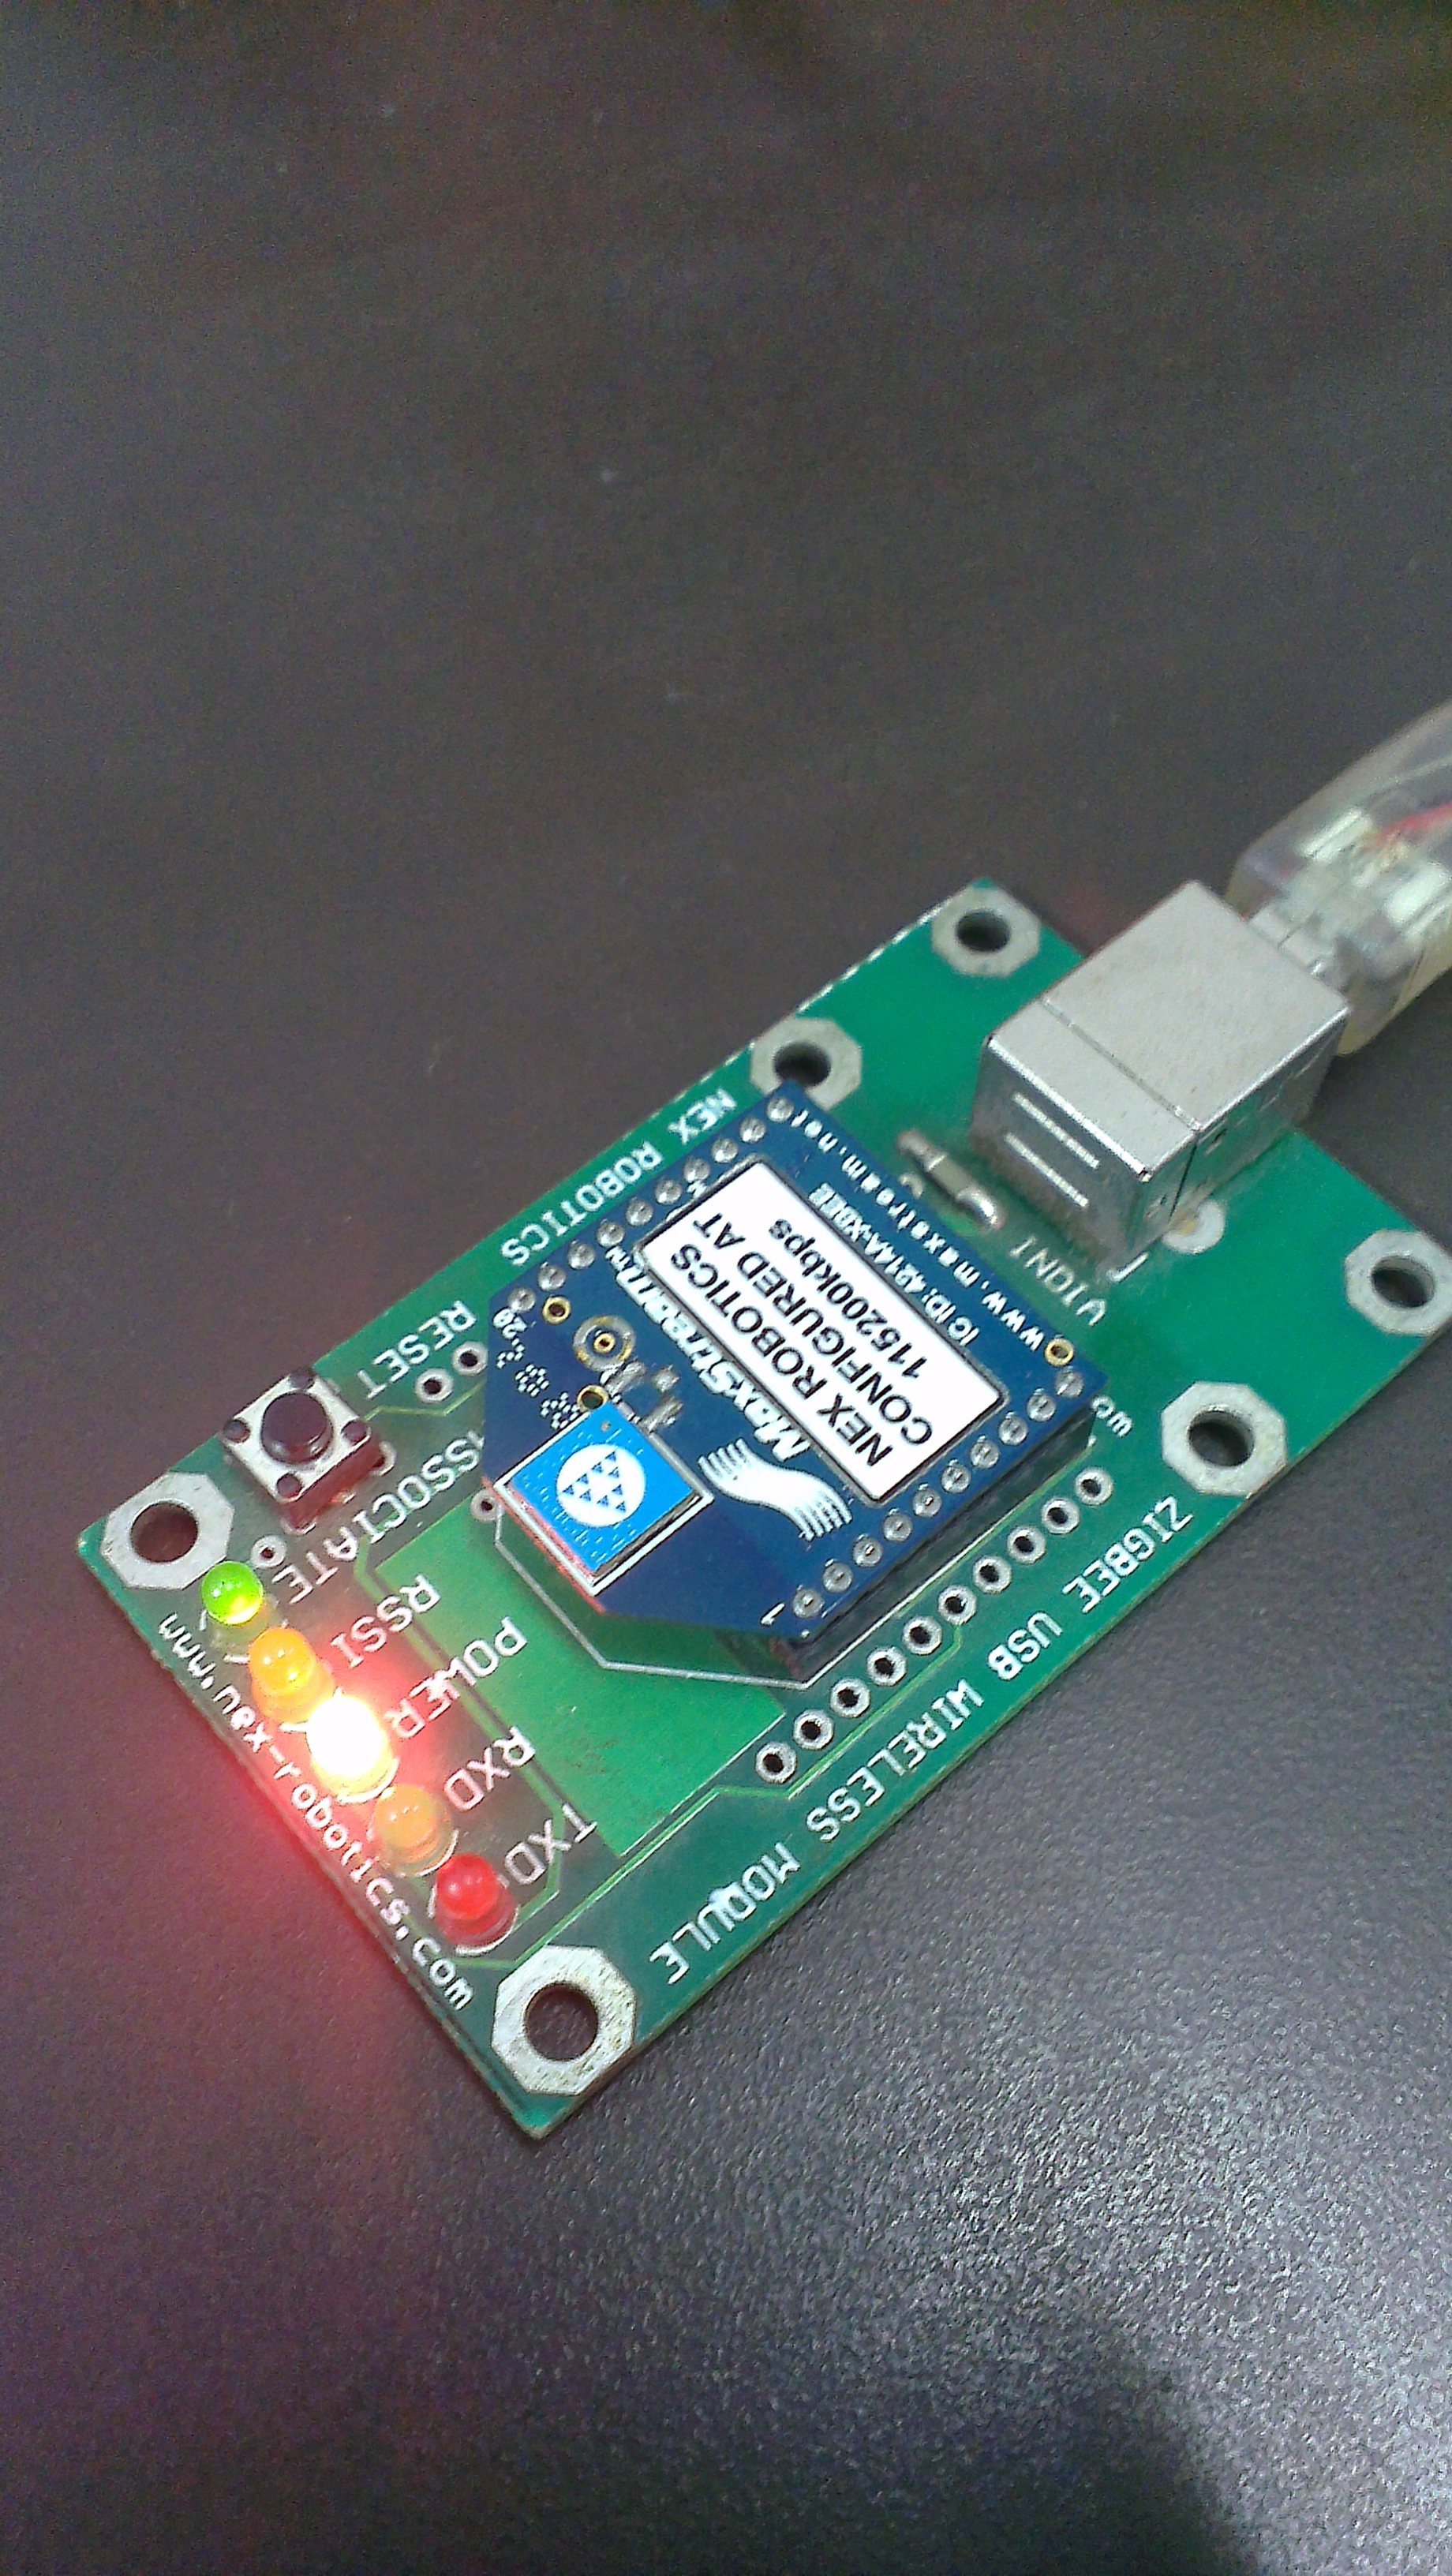
\includegraphics[scale=0.075]{zigbee_17}
\end{center}
\caption{Step 1(a) - Connecting XBee module with XBee USB adapter}
\label{xstep1.2}
\end{figure}

\newpage
\textbf{Step 2 :}
\medskip

Go to the "Modem Configuration" tab and click "Read" under "Modem Parameter and Firmware" section. The Modem Parameters will appear in the viewing area below. If they don't appear and such a pop-up comes up, press the "Reset" button on the Zigbee USB adapter and try reconnecting the adapter and then pressing the "Reset" button if it does not work.
Shown in figure \ref{xstep2}.

\medskip

\begin{figure}[h]
\begin{center}
\includegraphics[scale=0.5]{zigbee_11}
\end{center}
\caption{Step 2 - Reading the Modem Parameters}
\label{xstep2}
\end{figure}


\newpage

\textbf{Step 3 :}

\medskip

The parameters for both the XBee modules have to be set. Set the Channel and PAN ID of both the XBee modules as same. Set Destination Address High(DH) for both the modules as 0. The Destination Address Low(DL) and 16-bit Source Address(MY) have to be set such that the DL of one module is the MY of the other and MY of one module is the DL of other for both the modules. Here DL=2, MY=1 was used for the first module, and vice-versa for the other. 

\medskip
Configuration of the 2 Zigbee modules can be done one after another or simultaneously by launching 2 instances of X-CTU and connecting both the modules with the PC. Following these steps will configure the X-Bee modules in unicast mode, i.e. simple one-to-one wireless communication. It is recommended not to change the rest of the parameters and leave them at their default values. However, if you are an advanced user, you may tinker with their values if you know what you are doing.
Shown in figures \ref{xstep3.1} and \ref{xstep3.2} for both the modules.

\medskip

\begin{figure}[h]
\begin{center}
\includegraphics[scale=0.5]{zigbee_11}
\end{center}
\caption{Step 3(a) - Configuring the Modem parameters for XBee module 1}
\label{xstep3.1}
\end{figure}
\medskip

\begin{figure}[h]
\begin{center}
\includegraphics[scale=0.5]{zigbee_13}
\end{center}
\caption{Step 3(b) - Configuring the Modem parameters for XBee module 2}
\label{xstep3.2}
\end{figure}

\newpage

\textbf{Step 4 :}

After configuration of both the XBee modules, leave one of the modules in the USB Adapter and plug the other one in the Firebird V robot's X-Bee slot. Load the program "\_Interfacing\_Kinect\_To\_Firebird\_Using\_Zigbee.hex" provided with this document on the Firebird V robot. Start the X-CTU software and go to the "Terminal" tab.  You can send the byte sized commands shown in Table \ref{fbcommands} to the Firebird V robot to test the wireless connection via XBee: 

\medskip
\begin{figure}[h]
\begin{center}
\includegraphics[scale=0.1]{zigbee_16}
\end{center}
\caption{Step 4(a) - Connecting Zigbee module to Firebird V}
\label{xstep4.1}
\end{figure}
\medskip

\begin{figure}[h]
\begin{center}
\includegraphics[scale=0.5]{zigbee_14}
\end{center}
\caption{Step 4(b) - X-CTU's terminal Wizard}
\label{xstep4.2}
\end{figure}
\medskip

\begin{table}[h]
\begin{center}
\begin{tabular}{|c|c|c|}

\hline Keyboard Key & ASCII Value & Action \\ 
\hline 8 &  0x38 & Forward \\ 
\hline 2 &  0x32 & Backward \\ 
\hline 4 &  0x34 & Left \\ 
\hline 6 &  0x36 & Right \\ 
\hline 5 &  0x35 & Stop \\ 
\hline 7 &  0x37 & Buzzer On \\ 
\hline 9 &  0x39 & Buzzer Off\\  
\hline
\end{tabular}
\end{center}
\caption{Firebird V Commands}
\label{fbcommands}
\end{table}

\medskip

Congratulations! If you followed the above steps correctly, you just established a unicast connection between 2 X-Bee modules.
Shown in figure \ref{xstep4.1} and \ref{xstep4.2}.

\end{flushleft}
